% Generated by research/scripts/tables.py -- do not edit by hand.
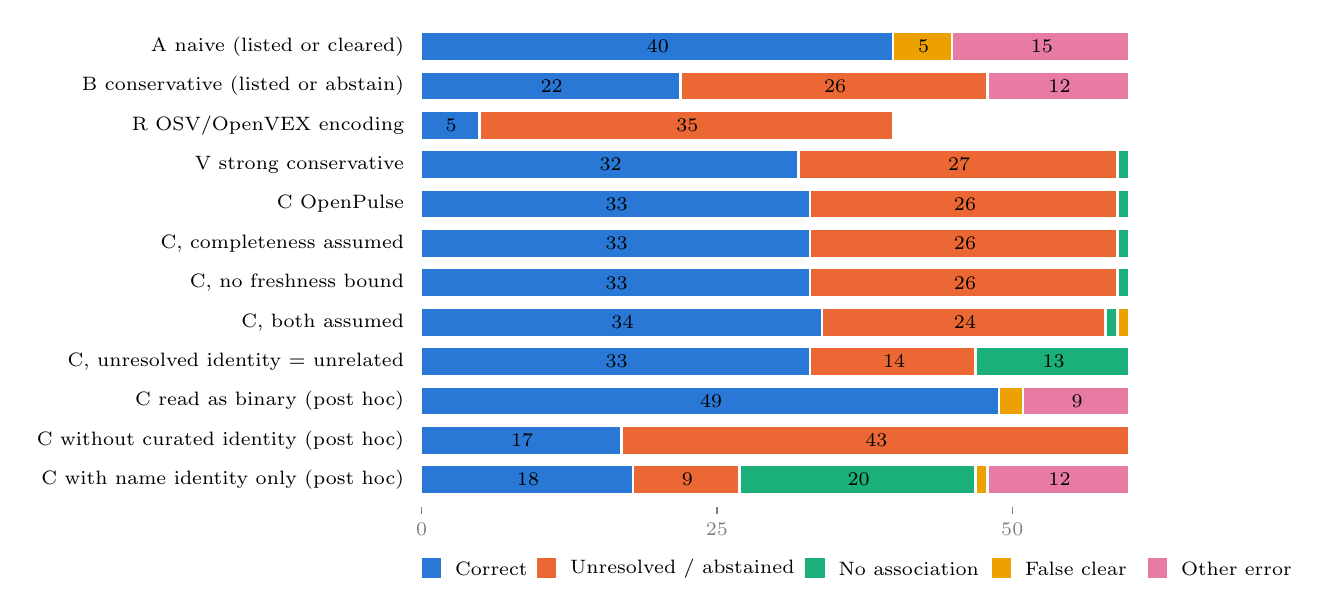
\begin{tikzpicture}[font=\scriptsize]
\definecolor{opcorrect}{HTML}{2A78D6}
\definecolor{opunresolved}{HTML}{EB6834}
\definecolor{opnoassociation}{HTML}{1BAF7A}
\definecolor{opfalseclear}{HTML}{EDA100}
\definecolor{opothererror}{HTML}{E87BA4}
\node[anchor=east] at (-0.1,-0.00) {A naive (listed or cleared)};
\fill[opcorrect] (0.000,-0.17) rectangle (5.970,0.17);
\node at (3.000,-0.00) {40};
\fill[opfalseclear] (6.000,-0.17) rectangle (6.720,0.17);
\node at (6.375,-0.00) {5};
\fill[opothererror] (6.750,-0.17) rectangle (8.970,0.17);
\node at (7.875,-0.00) {15};
\node[anchor=east] at (-0.1,-0.50) {B conservative (listed or abstain)};
\fill[opcorrect] (0.000,-0.67) rectangle (3.270,-0.33);
\node at (1.650,-0.50) {22};
\fill[opunresolved] (3.300,-0.67) rectangle (7.170,-0.33);
\node at (5.250,-0.50) {26};
\fill[opothererror] (7.200,-0.67) rectangle (8.970,-0.33);
\node at (8.100,-0.50) {12};
\node[anchor=east] at (-0.1,-1.00) {R OSV/OpenVEX encoding};
\fill[opcorrect] (0.000,-1.17) rectangle (0.720,-0.83);
\node at (0.375,-1.00) {5};
\fill[opunresolved] (0.750,-1.17) rectangle (5.970,-0.83);
\node at (3.375,-1.00) {35};
\node[anchor=east] at (-0.1,-1.50) {V strong conservative};
\fill[opcorrect] (0.000,-1.67) rectangle (4.770,-1.33);
\node at (2.400,-1.50) {32};
\fill[opunresolved] (4.800,-1.67) rectangle (8.820,-1.33);
\node at (6.825,-1.50) {27};
\fill[opnoassociation] (8.850,-1.67) rectangle (8.970,-1.33);
\node[anchor=east] at (-0.1,-2.00) {C OpenPulse};
\fill[opcorrect] (0.000,-2.17) rectangle (4.920,-1.83);
\node at (2.475,-2.00) {33};
\fill[opunresolved] (4.950,-2.17) rectangle (8.820,-1.83);
\node at (6.900,-2.00) {26};
\fill[opnoassociation] (8.850,-2.17) rectangle (8.970,-1.83);
\node[anchor=east] at (-0.1,-2.50) {C, completeness assumed};
\fill[opcorrect] (0.000,-2.67) rectangle (4.920,-2.33);
\node at (2.475,-2.50) {33};
\fill[opunresolved] (4.950,-2.67) rectangle (8.820,-2.33);
\node at (6.900,-2.50) {26};
\fill[opnoassociation] (8.850,-2.67) rectangle (8.970,-2.33);
\node[anchor=east] at (-0.1,-3.00) {C, no freshness bound};
\fill[opcorrect] (0.000,-3.17) rectangle (4.920,-2.83);
\node at (2.475,-3.00) {33};
\fill[opunresolved] (4.950,-3.17) rectangle (8.820,-2.83);
\node at (6.900,-3.00) {26};
\fill[opnoassociation] (8.850,-3.17) rectangle (8.970,-2.83);
\node[anchor=east] at (-0.1,-3.50) {C, both assumed};
\fill[opcorrect] (0.000,-3.67) rectangle (5.070,-3.33);
\node at (2.550,-3.50) {34};
\fill[opunresolved] (5.100,-3.67) rectangle (8.670,-3.33);
\node at (6.900,-3.50) {24};
\fill[opnoassociation] (8.700,-3.67) rectangle (8.820,-3.33);
\fill[opfalseclear] (8.850,-3.67) rectangle (8.970,-3.33);
\node[anchor=east] at (-0.1,-4.00) {C, unresolved identity = unrelated};
\fill[opcorrect] (0.000,-4.17) rectangle (4.920,-3.83);
\node at (2.475,-4.00) {33};
\fill[opunresolved] (4.950,-4.17) rectangle (7.020,-3.83);
\node at (6.000,-4.00) {14};
\fill[opnoassociation] (7.050,-4.17) rectangle (8.970,-3.83);
\node at (8.025,-4.00) {13};
\node[anchor=east] at (-0.1,-4.50) {C read as binary (post hoc)};
\fill[opcorrect] (0.000,-4.67) rectangle (7.320,-4.33);
\node at (3.675,-4.50) {49};
\fill[opfalseclear] (7.350,-4.67) rectangle (7.620,-4.33);
\fill[opothererror] (7.650,-4.67) rectangle (8.970,-4.33);
\node at (8.325,-4.50) {9};
\node[anchor=east] at (-0.1,-5.00) {C without curated identity (post hoc)};
\fill[opcorrect] (0.000,-5.17) rectangle (2.520,-4.83);
\node at (1.275,-5.00) {17};
\fill[opunresolved] (2.550,-5.17) rectangle (8.970,-4.83);
\node at (5.775,-5.00) {43};
\node[anchor=east] at (-0.1,-5.50) {C with name identity only (post hoc)};
\fill[opcorrect] (0.000,-5.67) rectangle (2.670,-5.33);
\node at (1.350,-5.50) {18};
\fill[opunresolved] (2.700,-5.67) rectangle (4.020,-5.33);
\node at (3.375,-5.50) {9};
\fill[opnoassociation] (4.050,-5.67) rectangle (7.020,-5.33);
\node at (5.550,-5.50) {20};
\fill[opfalseclear] (7.050,-5.67) rectangle (7.170,-5.33);
\fill[opothererror] (7.200,-5.67) rectangle (8.970,-5.33);
\node at (8.100,-5.50) {12};
\draw[gray] (0.000,-5.85) -- ++(0,-0.08) node[below] {0};
\draw[gray] (3.750,-5.85) -- ++(0,-0.08) node[below] {25};
\draw[gray] (7.500,-5.85) -- ++(0,-0.08) node[below] {50};
\fill[opcorrect] (0.00,-6.75) rectangle ++(0.25,0.25);
\node[anchor=west] at (0.30,-6.63) {Correct};
\fill[opunresolved] (1.46,-6.75) rectangle ++(0.25,0.25);
\node[anchor=west] at (1.76,-6.63) {Unresolved / abstained};
\fill[opnoassociation] (4.87,-6.75) rectangle ++(0.25,0.25);
\node[anchor=west] at (5.17,-6.63) {No association};
\fill[opfalseclear] (7.24,-6.75) rectangle ++(0.25,0.25);
\node[anchor=west] at (7.54,-6.63) {False clear};
\fill[opothererror] (9.22,-6.75) rectangle ++(0.25,0.25);
\node[anchor=west] at (9.52,-6.63) {Other error};
\end{tikzpicture}
